\documentclass[12pt]{report}

\usepackage[italian]{babel}
\usepackage[T1]{fontenc}
\usepackage[utf8]{inputenc}
\usepackage{algorithm}
\usepackage[noend]{algpseudocode}
\usepackage[pdftex]{graphics}
\usepackage{graphicx}
\graphicspath{/home/paologio/Documenti/Università/Tesi/Malchiodi/ACSDI/Elaborato}
\usepackage{chngcntr}
\counterwithout{footnote}{chapter}
\usepackage{booktabs}
\usepackage{cite}

\begin{document}

\tableofcontents

\chapter{Le reti neurali artificiali}

\linespread{1.4}\selectfont
\section{Definizione e origini storiche}
L’intuizione di replicare l’attività neurale che avviene nel sistema nervoso centrale umano quando apprende risale agli inizi degli anni ‘40, quando venne teorizzato un primo modello di neurone da McCulloch e Pitts (1943) ~\cite{McCulloch}. Il parallelo è molto stretto: così come il compito di un neurone è quello di ricevere, elaborare e ritrasmettere impulsi elettrici all’interno del sistema nervoso cerebrale, quello di un neurone artificiale è ricevere un certo dato in input e attivarsi o meno a seguito della sua elaborazione.
È interessante notare che, a differenza di un classico software, la costruzione di un neurone artificiale non richiede la scrittura di un programma ma avviene a seguito di un processo assimilabile a quello di apprendimento ~\cite{Perceptron}. Inoltre, continuando l'analogia con il sistema nervoso centrale, non ci si è limitati ad usare un singolo neurone ma più neuroni e più strati di neuroni collegati tra loro: questo ha portato allo sviluppo delle reti neurali.

\section{Il neurone artificiale}
Il neurone artificiale, vedi Figura 1.1, è composto da:
\begin{itemize}
\item{input}: rappresentati da $x_1$, $x_2$, $\dots$, $x_n$, sono l'input che riceve il neurone
\item{pesi}: rappresentati da $w_1$, $w_2$, $...$, $w_n$, sono i pesi associati alle singole connessioni tra input e neurone
\item{$\Sigma$}: viene eseguito $\displaystyle{\sum_{i=1}^n x_i \times w_i}$
\item{funzione d'attivazione}: la sommatoria al passo precedente viene usato come argomento per la funzione d'attivazione
\item{output}: il risultato dei passaggi precedenti viene propagato in output stabilendo l'attivazione o meno del neurone
\end{itemize}

\begin{figure}
\begin{center}
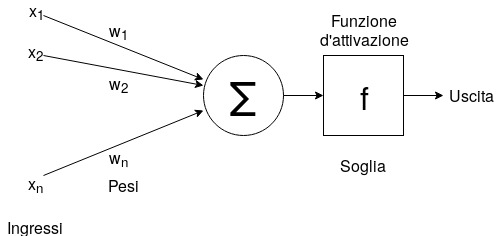
\includegraphics[scale=0.75]{neurone_artificiale.png}
\caption{Immagine di un neurone artificiale}
\end{center}
\end{figure}

\section{Architettura di una rete neurale}
Come detto precedentemente, una volta costruito un neurone artificiale, il passo successivo è stato quello di usare più neuroni in modo da formarne degli strati e connettere più strati tra di loro.
Una rete, per essere definita tale, deve essere composta da almeno 3 strati, vedi Figura 1.2:
\begin{enumerate}
\item{input}
\item{hidden}
\item{output}
\end{enumerate}

\begin{figure}
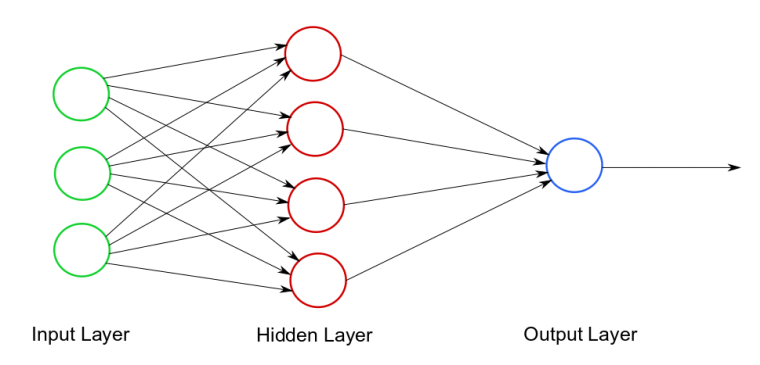
\includegraphics[scale=0.5]{nn_arch.png}
\caption{Architettura rete neurale}
\end{figure}

Il ruolo dello strato di input è quello di ricevere le feature da elaborare, lo strato nascosto si occuperà di rendere il modello più espressivo a livello di risoluzione di problemi di apprendimento rispetto ad uno con un solo neurone. Infine lo strato di output dovrà predire il risultato in base all’input ricevuto.

Inoltre, in base a come i neuroni dei vari strati sono collegati tra loro si possono distinguere due configurazioni di rete come quella densamente connessa (fully connected) o convoluzionale (convolutional) usate principalmente per il riconoscimento di pattern in immagini: a differenza di quelle densamente connesse, i neuroni di uno strato sono collegati solo ad una piccola parte dello strato precedente ~\cite{Convolutional}

In questo elaborato ci si concentrerà sulla tipologia densamente connessa, in cui ogni neurone di uno strato sarà collegato ad ogni neurone del successivo.

\subsection{Componenti}
Come detto sopra, la rete è composta da strati; gli strati, a loro volta, sono un insieme di neuroni, ognuno dei quali ha associato un peso ($w$) per ogni collegamento in entrata e un bias ($b$). Questi sono stati impostati randomicamente, in un intervallo tra 0 e 1. Questi due sono gli unici parametri che, una volta inizializzati, vengono modificati automaticamente dalla rete durante il training. I restanti parametri, come il numero di neuroni in uno strato hidden o il numero di strati, rimangono tali durante tutte le fasi di addestramento del modello; inoltre l'approccio tipicamente usato per individuare tali parametri è quello empirico: questi prendono il nome di \textit{iperparametri}.


\section{Applicazioni}
Le reti neurali vengono impiegate nell’attività di previsione (regressione) o classificazione.
Nel primo caso rientrano, ad esempio, le previsioni di vendita: riuscire a prevedere il prezzo di un immobile in base a fattori che lo descrivono (i metri quadrati, il numero di stanze, la posizione centrale o meno in un centro abitato, ecc…) o prevedere l’andamento di un titolo azionario in borsa.
Altro problema è quello invece della classificazione: si richiede in questo caso che la rete, dato un oggetto, ne restituisca la classe di appartenenza; tipico esempio è quello della classificazione di numeri scritti a mano o, date una serie di immagini, riconoscere quelle in cui è presente un particolare soggetto.
In questo elaborato si andrà ad affrontare il problema legato alla regressione.

\section{Esecuzione di una rete feed-forward}
Le connessioni tra i neuroni di uno strato e quelli del successivo sono monodirezionali, configurazione che porta ad avere un grafo diretto e aciclico. Quindi il flusso di dati che scorre nella rete viaggia dallo strato di input a quello di output senza che ci siano loop, il che implica anche che non ci siano interazioni tra neuroni dello stesso strato e che il tempo necessario per far scorrere i dati da input a output è costante.

\subsection{Il calcolo tra strati}\label{feedforward}
Nell'implementazione pratica vengono usate delle matrici dei pesi per rappresentare le connessioni tra strati e dei vettori per rappresentare i valori di bias dei pesi . 
Siano 
\begin{itemize}
\item{$W_{ih}$} la matrice dei pesi che rappresenta le connessioni tra strato input e hidden;
\item{$W_{ho}$} la matrice dei pesi che rappresenta le connessioni tra strato hidden e output;
\item{$b_h$} il vettore dei bias dello strato hidden;
\item{$b_o$} il vettore dei bias dello strato di output;
\item{$x$} il vettore di input;
\item{$f$} la funzione d'attivazione scelta per lo strato.
\end{itemize}
Per eseguire l'algoritmo di feed-forward occorre calcolare
$$\alpha = f\left(x \cdot W_{ih} + b_h\right),$$
procedendo poi analogamente con lo strato successivo
$$\mathrm{prediction} = f\left(\alpha \cdot W_{ho} + b_o\right).$$
Le reti considerate in questo lavoro vengono utilizzate per calcolare una regressione, e dunque hanno un solo neurone di output: prediction sarà quindi un valore scalare che rappresenterà la previsione della rete in base all'input ricevuto.

\section{Addestramento di una rete neurale}
Per continuare il parallelo con il sistema nervoso centrale umano, così come per l'attività di apprendimento occorre studiare, anche una rete neurale artificiale ha bisogno di ''studiare``: questa fase viene detta fase di addestramento (training).
Una volta selezionato il dataset contenente i caratteri che la rete dovrà apprendere, si procede a dividere tale insieme in due sottoinsiemi:

\begin{itemize}
\item{training set};
\item{testing set}.
\end{itemize}

Il primo verrà usato per l'attività di apprendimento, il secondo per valutare la bontà della rete su esempi che non ha ancora visto. Per selezionare la quantità di dati tra i due insiemi è stato utilizzato un holdout di 80\% - 20\%; una soluzione alternativa sarebbe stata quella di fare una cross-validation.

\subsection{Fase di training}
In questa fase le feature degli esempi nel training set vengono copiate nello strato di input della rete. Utilizzando la procedura descritta nel Paragrafo \ref{feedforward} la rete propaga il risultato fino al neurone di output. È in questo momento che la rete impara confrontando la previsione con l’effettivo target: in base alla loro differenza, la rete stessa correggerà i pesi degli strati usando un algoritmo noto come back-propagation (spiegato nel Paragrafo \ref{backprop}).
Questa operazione viene eseguita un numero n di volte, numero che prende il nome di epoca. Questo parametro indica che la rete ha visto tutti gli esempi del training set. Il concetto di epoca è strettamente legato a quello di batch size, iperparametro che specifica dopo ogni quanti esempi i pesi della rete verranno aggiornati.
Esempio: se avessi 200 esempi nel training set, batch size pari a 10 e 100 epoche significherebbe che in un epoca avverranno 20 aggiornamenti ($200 \div 10$) e al termine delle epoche 2000 aggiornamenti ($20 \times 100$).
Una volta che la rete ha iterato per un numero pari al numero di epoche scelto termina la fase di training.

Inoltre esistono diversi criteri per stabilire quando terminare l'apprendimento; in particolare negli esperimenti condotti in questo elaborato ne sono stati usati due basati su:
\begin{itemize}
\item{epoche}: il processo di apprendimento prosegue fino al raggiungimento del numero di epoche predefinito;
\item{valore della loss function}: vengono fissate due soglie, $s_1$ e $s_2$; l'apprendimento termina quando la loss function non supera $s_1$ per $s_2$ volte consecutive.
\end{itemize}

\subsection{Fase di testing}
Terminata la fase di training occorre verificare il comportamente della rete su dati nuovi rispetto a quelli usati per addestrarla. Questo permette di capire la reale capacità di previsione della rete e di valutare se durante l'addestramento si sia verificato uno dei problemi descritti di seguito.
\begin{itemize}
\item{Si parla di \textit{overfitting} quando il modello si adatta così tanto agli esempi del training set da perdere la capacità di generalizzare su nuovi esempi. Sintomo dell'overfitting è un'alta accuratezza durante la fase di training e una scarsa accuratezza in fase di testing; la rete ha imparato ''a memoria`` i casi di training in modo tale da non riconoscerne di nuovi};
\item{L'\textit{underfitting} è l'opposto del caso precedente. Si verifica quando il modello non riesce ad imparare la relazione tra feature e target, risultando in previsioni poco accurate}.
\end{itemize}

\section{Algoritmo di back-propagation}\label{backprop}
Una volta che l’informazione ha raggiunto lo strato di output ho la previsione; tuttavia questa conterrà dell’errore. Per ridurlo si usa un apposito algoritmo di propagazione all’indietro che regola i pesi associati ai collegamenti tra singoli neuroni, partendo dallo strato più esterno a quello più interno.

Si parte calcolando la loss function dell’output, che può essere l’errore medio assoluto (scelta fatta per gli esperimenti dell'elaborato) o l’errore quadratico medio, e se ne calcola la derivata parziale rispetto ai pesi dei collegamenti dei neuroni di output. A questo risultato si moltiplica il learning rate e si sottrae al peso $$W^n_x = W_x - \eta \left(\frac{\delta Error}{\delta W_x}\right)$$ dove $W^n_x$ è il valore del nuovo peso, $W_x$ il vecchio peso, $\eta$ il learning rate e tra parentesi $\frac{\delta Error}{\delta W_x}$ la derivata parziale dell'errore rispetto ai pesi. 

Una volta fatto questo calcolo con la matrice dei pesi strato hidden/output, si fa la stessa cosa per quella input/hidden.

\subsection{Iperparametri}\label{iperparametri}
Gli iperparametri sono tutti quelli il cui valore viene impostato prima che l'addestramento abbia inizio e che non cambiano nel corso dello stesso. Negli esperimenti presentati in questo elaborato questi valori vengono cercati empiricamente attraverso model selection (vedi \ref{modelselection})
In questa categoria rientrano:
\begin{itemize}
\item{learning rate}: indica il grado con cui la rete modifica i propri pesi durante la fase di back-propagation;
\item{numero di epoche}: indica il numero di volte che la rete ha visto tutti gli esempi del training set;
\item{batch size}: indica dopo quanti esempi mostrati alla rete si aggiornano i pesi;
\item{numero di neuroni per strato per strato nascosto}: indica il numero di neuroni per singolo strato;
\item{funzione d'attivazione}: funzione che determina l'intensità d'attivazione del singolo neurone.
\end{itemize}

Ogni volta che in questo elaborato verranno introdotti nuovi esperimenti ne verranno anche indicati gli iperparametri coinvolti.

\section{Model selection}\label{modelselection}
Come indicato nel paragrafo \ref{iperparametri}, per trovare il valore degli iperparametri bisogna basarsi su prove empiriche. In particolare, negli esperimenti condotti sono stati fissati a priori i valori per numero di epoche, batch size, numero di strati nascosti, learning rate e funzione d'attivazione. Il numero di neuroni dello strato nascosto è stato dimensionato usando una tecnica di model selection che prende il nome di cross-validation annidata e che è spiegata nel prossimo paragrafo.

\subsection{Cross validation annidata}
Dopo aver diviso il training set dal testing set, viene utilizzato esclusivamente  il primo per la cross-validation. In particolare questo viene partizionato in $k$ sottoinsiemi (fold) di cui uno di questi prenderà il nome di validation set e gli altri di training set. Per ogni valore possibile dell'iperparametro (o per ogni possibile configurazione se ci sono più iperparametri) vengono ripetuti $k$ processi di addestramento, ogni volta eliminando dal training set uno dei fold e utilizzando quet'ultimo per calcolare l'errore; si ottengono così $k$ errori di cui si calcola la media.

\newpage
Es.: se il training set venisse suddviso in 3 fold le permutazioni prese in considerazione saranno:
\begin{enumerate}
\item{TRAINING | TRAINING | VALIDATION}
\item{TRAINING | VALIDATION | TRAINING}
\item{VALIDATION | TRAINING | TRAINING}
\end{enumerate}

Viene infine scelto il valore che corrisponde all'errore medio minore, e si riaddestra una rete dopo aver fissato a quel valore l'iperparametro.

Quella spiegata è la procedura di cross-validation: tuttavia quella usata in questo elaborato è una tipologia innestata. Quello che cambia è che, le operazioni viste sopra, che ora prenderanno il nome di fold interno, vengono ripetute j volte, dove j è il numero di fold esterno. Di seguito è presentato lo pseudo codice per una procedura di nested-cross-validation.

\makeatletter
\def\BState{\State\hskip-\ALG@thistlm}
\makeatother

\begin{algorithm}
\caption{Nested Cross Validation}
\begin{algorithmic}[1]
\Procedure{NestedCrossValidation}{}
\BState \emph{input}:
\State $H \gets \textit{insieme di iperparametri presi in considerazione}$
\State $S \gets \textit{training set}$
\State $K \gets \textit{numero di fold esterni}$
\State $J \gets \textit{numero di fold interni}$
\BState \emph{procedure}:
\State $S_{perm} \gets \textit{K permutazioni di S}$
\For {$k \in \{1,\dots,K\}$}
\State $s_{k} \gets \textit{k-esima permutazione di S}$
\State $L_M \gets \infty$

\For {$h \in H$}
\For {$j \in \{1, \dots, J\}$}
\State $s_{kj} \gets \textit{singola permutazione kj}$
\State $\textit{alleno la rete sul training set di} s_{kj}$
\State $\textit{valuto la rete sul validation set di} s_{kj}$
\State $L_j \gets \textit{valore di loss per il j-esimo fold}$
\EndFor
\State $L_{mean} \gets \textit{media delle loss} L_j$
\State $L_M \gets L < L_{mean} ? L : L_{mean}$
\EndFor
\State $Best[k] \gets \textit{risultato migliore per il k-esimo fold}$
\EndFor
\State $\textit{Per ogni iperparametro ho il carattere migliore dei k fold}$
\EndProcedure
\end{algorithmic}
\end{algorithm}

\chapter{Algoritmi di compressione per reti neurali}

\section{Compressione di una rete}

Uno degli svantaggi più evidenti delle reti neurali è lo spazio che queste occupano in memoria e i tempi elevati per il loro l’addestramento. Questo aspetto ha assunto un ruolo sempre più importante con il diffondersi di macchine con ridotte capacità di computazione e di memoria e in generale dell’IoT. 
Per ridurre questo impatto negativo si stanno studiando diversi metodi per comprimere le strutture dati alla base di una rete neurale in modo da ridurne le dimensioni in memoria lasciando il più possibile invariata l’accuratezza. Questo elaborato si prefigge di verificare l'efficacia di due tecniche di compressione note come ''pruning`` e ''weight sharing`` su una rete neurale feed-forward utilizzata per problemi di regressione.

\section{Pruning}

L’idea di fondo del pruning è semplice: ogni collegamento tra neuroni ha associato un peso che ne determina l’importanza (avrà letteralmente un peso maggiore nell’influenzare il risultato finale della rete quando il valore della connessione è molto alto o molto basso), da qui l’intuizione per cui, ignorando i collegamenti con peso tendente allo zero, non altero significativamente il risultato della rete che otterrei considerandoli. 
Si sceglie quindi di annullare queste connessioni rendendo così sparsa la matrice dei pesi da memorizzare. Tuttavia questa operazione non è del tutto gratuita: ci si ritrova con nuove strutture dati per le quali è più lenta l'operazione di moltiplicazione tra matrici. Due scelte possibili per la struttura dati che accoglie la matrice sparsa sono indicate di seguito.
\begin{itemize}
\item{\textbf{\textit{compressed Sparse Row}}}: vengono usati 3 vettori contenenti rispettivamente i valori non non nulli della matrice, letti riga per riga, un puntatore alle righe e gli indici di colonna;
\item{\textbf{\textit{compressed Sparse Column}}}: simile alla precedente con la differenza che nel primo vettore i valori vengono letti per colonna, vengono memorizzati gli indici di riga per ogni valore e i relativi puntatori alle colonne.
\end{itemize}


In questo elaborato la soglia per scartare i pesi è stata calcolata come $n$-esimo percentile rispetto alla distribuzione dei pesi nella matrice, per $n \in \{10, \dots, 90 \}$ (quindi per $n=10$ verranno scartate il 10\% circa delle connessioni tra due strati comunicanti e così via).

\section{Weight Sharing}

L’obiettivo del weight sharing è quello di ridurre lo spazio necessario alla memorizzazione delle matrici dei pesi della rete; per fare ciò si raggruppano pesi simili in un singolo valore che riesca a rappresentarli adeguatamente. Questo valore prende il nome di centroide e verrà usato in sostituzione ai pesi raggruppati per le operazioni matriciali. 

Per stabilire i centroidi si possono usare algoritmi di clustering; in particolare quello usato in questo elaborato è K-Means, che verrà spiegato nel dettaglio nel Paragrafo \ref{kmeans}. Per gli esperimenti trattati nell'elaborato, dopo aver fissato il numero di clusters per strato e dopo averne trovato i centroidi, le matrici dei pesi sono state sostituite con le matrici di indici che puntano al relativo centroide. 

\subsection{Algoritmo K-Means}\label{kmeans}
K-Means
L’algoritmo usato è quello della libreria sklearn, MiniBatchKMeans, che da documentazione segue l’euristica di Lloyd, descritta di seguita.

\begin{enumerate}
\item{Vengono scelti k centroidi casualmente, dove k è il numero di clusters che si vogliono creare}.
\item{Ogni osservazione viene assegnata ad uno dei centroidi in base alla distanza euclidea dello stesso}.
\item{I centroidi vengono aggiornati in base alla media dei valori rientranti nel cluster}.
\item{Se i centroidi sono stati aggiornati si ripete iterativamente dal punto 2, altrimenti l’algoritmo ha trovato i k centroidi}.
\end{enumerate}
 

\chapter{Esperimenti}

L'obiettivo di questo tirocinio è quello di verificare l'efficacia di tecniche di compressione su una rete neurale col compito di risolvere il problema del predecessore \ref{probPred}.
Si è deciso di cominciare focalizzandosi sul problema della regressione: è stato usato un dataset con informazioni relative alle caratteristiche dei giocatori di calcio Fifa 2019 \footnote{https://www.kaggle.com/karangadiya/fifa19, ultimo controllo ...} con l’obiettivo di predire il valore di mercato del giocatore. Per questa fase sono state usate due tipi di reti: la prima sfruttando le API di Keras, la seconda è stata creata ad hoc per essere successivamente compressa.

Una volta conclusa questa parte si è affrontato il problema della compressione per il problema del predecessore usando un dataset contenente gli elementi ordinati come feature, e la relativa funzione di ripartizione empirica come target.

D'ora in poi si utlizzerà il termine feature per indicare una caratteristica che la rete usa durante la fase di training per predire il risultato e target per indicare il valore da predire in base alle feature in input.

\section{Dataset utilizzati}

\subsection{Fifa 2019}

Il primo dataset utilizzato è stato quello dei giocatori fifa, composto da 89 feature e circa 18.2k esempi. 
Una volta eliminate le feature non necessarie all’esperimento (nome del giocatore, immagine del club, numero di maglia, ecc… ) si è proceduto a convertire tutti i valori numerici rappresentati come stringhe (come “Value”, “Release clause”, “Height”, ecc…) in float e a rimuovere dal dataset tutti gli esempi il cui “Value” risultasse superiore o uguale al valore minimo tra gli outlier trovati \footnote{SPIEGARE COME SONO STATI CALCOLATI GLI OUTLIER}. Inoltre i nomi delle squadre di appartenenza sono stati inclusi come feature significative e codificati in interi.

Terminata questa fase preliminare si è deciso di considerare diverse alternative: la prima in cui vengono considerate tutte le feature a disposizione, la seconda in cui vengono selezionate solamente quelle il cui indice di correlazione \footnote{Calcolato tramite il metodo corr di pandas che utilizza il coefficiente di correlazione di Pearson $\rho_{X,Y} = \frac{cov(X, Y)}{\sigma_X\sigma_Y}$ dove $cov$ è la covarianza, $\sigma_X$ la deviazione standard di X e $\sigma_Y$ la deviazione standard di Y} fosse maggiore di 0.55.
È stata considerata anche una terza opzione: selezionare la metà delle feature tramite la Principal Component Analysis (PCA) scegliendo di mantenere la metà delle feature. 

\subsection{Problema del predecessore}\label{probPred}
Data una lista di interi ordinata e un intero, predire l'indice del predecessore di quest'ultimo. In questa versione semplificata non si prendono in considerazione elementi diversi da quelli già presenti nella lista e si considera solamente il problema del posizionamento tralasciando quello di inserimento e cancellazione di un elemento.
Il problema viene affrontato addestrando la rete a predire, in base all'elemento, il valore della sua funzione di ripartizione empirica in modo poi da essere in grado di ottenere l'indice del predecessore tramite $$index=\lceil\hat{F}(x)\times n\rceil$$

\section{Architettura della rete}
La prima rete considerata è stata costruita sfruttando delle API di Keras (che a sua volta usa Tensorflow come backend). La rete è composta da uno strato di input con un numero di neuroni pari al numero di feature considerate, uno strato hidden con N neuroni e uno strato di output con un singolo neurone. Per gli iper-parametri si è deciso di fissare learning rate, numero di epoche, batch size e funzione d'attivazione; per trovare il numero di neuroni per il singolo strato hidden, invece, si è usata una tecnica di model selection, modalità descritta precedentemente, quella della nested cross-validation.

\subsection{Oragnizzazione dei dati}
Una volta mescolati gli esempi randomicamente, sono stati estratti l'80\% degli esempi come training set e il restante 20\% per il testing set. Inoltre entrambi i set sono stati ulteriormente divisi in X\_train e X\_test (contenente solo le colonne di feature) e y\_train e y\_test (contenente solo il target, cioè “Value”). Ogni valore null all’interno dei set è stato poi sostituito con la media della relativa colonna e i valori scalati usando StandardScaler di sklearn che utilizza la seguente formula
$$z = \frac{x - u}{s}$$ 
dove u è la media del campione e s è la deviazione standard del campione.

\subsection{Addrestramento}
Per scegliere il giusto numero di neuroni per lo strato hidden si è proceduto con una cross-validation innestata. Di seguito vengono riportati gli iper-parametri scelti per la rete:
\begin{itemize}
\item{funzione d’attivazione}:

\begin{itemize}
\item{ReLu 
\footnote{$f(x) =
\bigg \{
\begin{array}{rl}
x & x > 0 \\
0 & x \leq 0 \\
\end{array}
$
} per i neuroni dello strato hidden};
\item{lineare per il neurone d'output};
\end{itemize}

\item{loss function}: errore medio assoluto \footnote{
$\displaystyle{\frac{\sum_{i=1}^n \left|x_i - y_i\right|}{n}} \; \textit{dove x è l'i-esimo valore predetto, y è l'i-esimo target}$
};

\item{ottimizzatore}: Adam (componente Keras) con

\begin{itemize}
\item{learning rate}: 0.001;
\item{beta\_1}: 0.9;
\item{beta\_2}: 0.99;
\item{decay}: 0.0;
\end{itemize}

\item{numero epoche}: 100;

\item{batch size}: 125 esempi.
\end{itemize}

Il numero di fold esterni è stato impostato a 3 e quello interno a 5, provando per l'unico hidden layer un numero di neuroni tra 10 e 200 a step di 10.

\section{Risultati}

\subsection{Rete Keras}

I risultati migliori per singolo fold, considerando tutte le feature, sono
\begin{center}
\begin{tabular}{lcr}
\toprule
Fold & Accuracy & Neurons \\
\midrule
1  & 0.9936 & 200\\
2  & 0.9921 & 190\\
3  & 0.9916 & 200\\
\bottomrule
\end{tabular}
\end{center}

\par\null\par
\par\null\par

I risultati migliori per singolo fold, considerando solo le feature con correlazione superiore a 0.55, sono

\begin{center}
\begin{tabular}{lcr}
\toprule
Fold & Accuracy & Neurons \\
\midrule
1  & 0.9723 & 200\\
2  & 0.9691 & 160\\
3  & 0.9696 & 200\\
\bottomrule
\end{tabular}
\end{center}

\par\null\par
\par\null\par

I risultati migliori per singolo fold, considerando le feature selezionate con PCA, sono

\begin{center}
\begin{tabular}{lcr}
\toprule
Fold & Accuracy & Neurons \\
\midrule
1  & 0.9933 & 180\\
2  & 0.9924 & 200\\
3  & 0.9922 & 180\\
\bottomrule
\end{tabular}
\end{center}

\par\null\par

Osservato il risultato migliore in corrispondenza del numero massimo di neuroni si è deciso di inserire un ulteriore strato hidden riducendo l'intervallo di neuroni in fase di cross validation, da 10 a 40.
Inoltre si è deciso di proseguire considerando tutte le feature.

I risultati migliori per singolo fold, considerando tutte le feature, sono

\par\null\par

\begin{center}
\begin{tabular}{lcr}
\toprule
Fold & Accuracy & Neurons \\
\midrule
1  & 0.9951 & 40, 40\\
2  & 0.9947 & 40, 40\\
3  & 0.995 & 40, 40\\
\bottomrule
\end{tabular}
\end{center}

\par\null\par
\par\null\par

I risultati migliori per singolo fold, considerando le feature selezionate tramite PCA, sono

\par\null\par

\begin{center}
\begin{tabular}{lcr}
\toprule
Fold & Accuracy & Neurons \\
\midrule
1  & 0.9951 & 40, 40\\
2  & 0.9947 & 40, 40\\
3  & 0.995 & 40, 40\\
\bottomrule
\end{tabular}
\end{center}

\par\null\par
\par\null\par

\subsection{Rete ad hoc}
Purtroppo la rete costruita usando le API di Keras non si presta alla manipolazione necessaria per la compressione, né per il pruning, non c’è modo per mantenere inattive le connessioni tagliate, né per il weight sharing, non c’è compatibilità con le nuove strutture dati necessarie alla tecnica stessa.
Si è quindi proceduto alla costruzione di una rete simile che si prestasse alla compressione. Come per la rete precedente si sono usati gli stessi iper-parametri eccezion fatta per il numero di neuroni dello strato nascosto: per questi si è proceduto con una nested-cross-validation considerando prima un numero di neuroni compreso tra 10 e 40 ad intervalli di 10 e poi tra 10 e 100 ad intervalli di 10.
Di seguito sono riportati i risultati.

\par\null\par

\begin{center}
\begin{tabular}{lcr}
\toprule
Fold & Accuracy & Neurons \\
\midrule
1  & 0.9941 & 40, 40\\
2  & 0.9938 & 40, 40\\
3  & 0.993 & 40, 30\\
\bottomrule
\end{tabular}
\end{center}

\par\null\par

\begin{center}
\begin{tabular}{lcr}
\toprule
Fold & Accuracy & Neurons \\
\midrule
1  & 0.9939 & 100, 100\\
2  & 0.994 & 80, 90\\
3  & 0.9934 & 90, 100\\
\bottomrule
\end{tabular}
\end{center}

\bibliography{bibliography}{}
\bibliographystyle{unsrt}

\end{document}
